\documentclass[tikz,border=5pt]{standalone}
\begin{document}
\def\blockW{0.8}
\def\blockH{1.2}
\def\tmpx{\blockW}
\def\tmpy{\blockH}
\def\origin{\blockW}
\NewDocumentCommand\mydraw{ O{} m }{
    \draw[#1,rotate around={-#2:(\origin,0)}] (\origin,0) rectangle ++(-\tmpx, \tmpy);
    \ifnum#2=90\relax
        \pgfmathparse{\origin + \tmpy}
        \global\let\origin\pgfmathresult
        \global\let\tmp\tmpx
        \global\let\tmpx\tmpy
        \global\let\tmpy\tmp
        % \fill[red] (\origin,0) circle (2pt);
    \fi
}
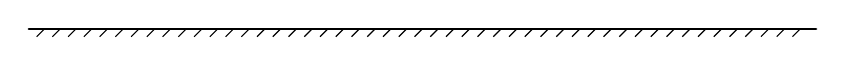
\begin{tikzpicture}
        \foreach \nn/\mycolor in {
            1/magenta,
            2/cyan,
            3/orange,
            4/violet,
            5/purple,
            6/teal,
            7/lime,
            8/black%
        } {%
            \foreach \ang in {45,75,90}{\mydraw[\mycolor!\ang]{\ang}}
        }
    \draw[thick,line cap=round] (0,0) -- (10,0);
    \foreach \x in {.2,.4,...,9.8}
        \draw (\x,0) -- ++(-.1,-.1);
\end{tikzpicture}
\end{document}